\documentclass[11pt,a4paper]{article}

\usepackage{style2017}
\usepackage{hyperref}

\hypersetup{
    colorlinks =false,
    linkcolor=blue,
   linkbordercolor = 1 0 0
}
\newcounter{numexo}
\setcellgapes{1pt}

\begin{document}



\begin{NSI}
{Exercice}{Requête HTTP}
\end{NSI}

\addtocounter{numexo}{1}
\subsection*{\Large Exercice \thenumexo}

\begin{minipage}{9cm}
On donne la capture des en-têtes d'une requête HTTP effectuée par un navigateur.


\begin{enumerate}
\item Quelle est la méthode utilisée par cette requête ?
\item La ressource demandée a-t-elle été renvoyée par le serveur ? Justifier.
\item Quelle est la taille des données ?
\item Quel est le type de données envoyées par le serveur?
\item Quel est le domaine du site visité ?
\item Quelle est l'url affichée dans la barre d'adresse du navigateur ?
\item Quel est le serveur web utilisé par ce site?
\end{enumerate}
\vspace*{2.4cm}
\end{minipage}\hfill
\begin{minipage}{9cm}
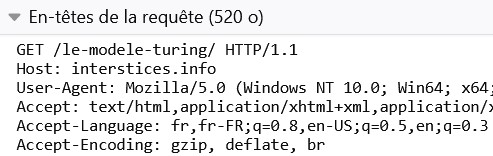
\includegraphics[scale=0.7]{img/req3Ex1.jpg}

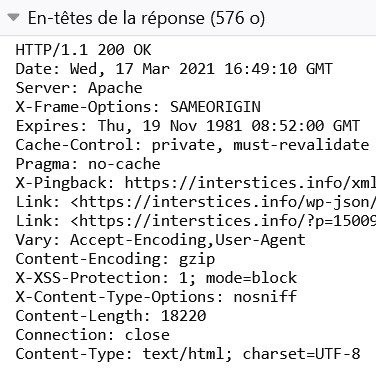
\includegraphics[scale=0.7]{img/req4Ex1.jpg}
\end{minipage}

%
%\addtocounter{numexo}{1}
%\subsection*{\Large Exercice \thenumexo}
%\begin{minipage}{9cm}
%On donne la capture d'une requête HTTP effectuée par un navigateur le 17 mars 2021.
%
%
%\begin{enumerate}
%\item Quelle est la méthode utilisée par cette requête ?
%\item Que signifie le code d'état \textbf{304 Not modified} ?
%\item Quelle est l'url du site visité ? de la page visitée ?
%\item Quel est le serveur web utilisé par ce site?
%\end{enumerate}
%\vspace*{3cm}
%\end{minipage}\hfill
%\begin{minipage}{9cm}
%\begin{center}
%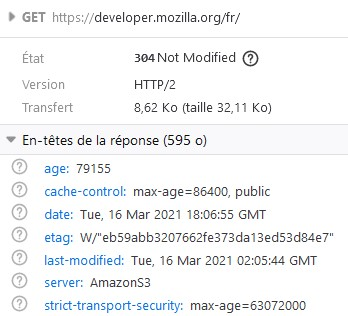
\includegraphics[scale=0.9]{img/req2Ex2.jpg}
%\end{center}
%\end{minipage}
%
%\newpage


\addtocounter{numexo}{1}
\subsection*{\Large Exercice \thenumexo}
\begin{minipage}{9cm}
On donne la capture d'une requête HTTP effectuée par un navigateur.
\begin{enumerate}
\item Quelle est la méthode utilisée par cette requête ?
\item Des données ont été envoyées au serveur par le client. Combien et comment ?
\item Quelle réponse a été fournie par le serveur et sous quelle forme?
\item On peut effectuer cette requête avec la méthode GET. Comment se réalise-t-elle ?
\end{enumerate}
\vspace*{4.5cm}
\end{minipage}\hfill
\begin{minipage}{9cm}
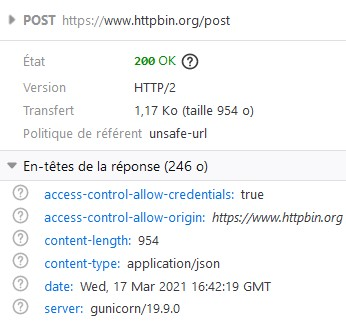
\includegraphics[scale=0.9]{img/reqEx3.jpg}

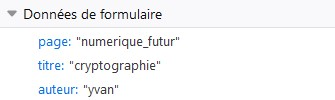
\includegraphics[scale=0.9]{img/req2Ex3.jpg}
\end{minipage}


\newpage

\addtocounter{numexo}{1}
\subsection*{\Large Exercice \thenumexo}
Le logiciel \textbf{curl} ou \textbf{cURL} est une application multi-plateforme. Cette application est un client HTTP qui effectue des requêtes HTTP en ligne de commande.

Cette application s'exécute avec différentes options:
\begin{itemize}
\item \textbf{curl -i} : Affiche le contenu complet de la réponse HTTP. On visualise ainsi la ligne de statut et les en-têtes retournés par le serveur.
\item \textbf{curl -I} : Affiche l'en-tête de la réponse HTTP retourné par le serveur.
\item \textbf{curl -v} : Mode verbeux affichant notamment la requête émise et la réponse reçue.

\item \textbf{curl -X [méthode]} : Permet de préciser la méthode HTTP à utiliser dans la requête (GET par défaut).

\item \textbf{curl -H "[en-tête]"} : Permet d'ajouter ou de modifier un en-tête de la requête.

\item \textbf{curl -{}-data-binary [data]} : Ajoute les données spécifiées comme corps du message

\item \textbf{curl -o [nom de fichier]} : Permet de sauvegarder la réponse retournée par le serveur dans un fichier. 
\end{itemize}
\begin{enumerate}
\item Ouvrez l'application \textbf{cmd} de windows et vérifier que le logiciel \textbf{curl} est bien installé en tapant la commande \textbf{curl -{}-version}.
\item \begin{enumerate}
\item Effectuer une requête HTTP vers l'adresse https://interstices.info et afficher l'en-tête de la réponse HTTP.
\item Enregistrer la page d'accueil du site avec curl et ouvrez-là dans un navigateur.
\end{enumerate}
\item Choisissez une image ou photo sur le site \textbf{wikimedia commons} et en récupérer son url.
\begin{enumerate}
\item Effectuer une requête HTTP avec curl sur cette image pour en récupérer sa taille en octets.
\item Enregistrer cette image avec curl. Vérifier le fichier et sa taille en octets.
\item Enregistrer l'image en utilisant le navigateur. A-t-on la même taille ?
\end{enumerate}
\item Parmi les adresses suivantes, donner les codes d'état des réponses HTTP suite à une requête HTTP avec curl sur les url suivantes:
\begin{enumerate}
\item http://oups.fr
\item https://faillite.com
\item http://cretin.fr
\item https://www.fier-comme-un-coq.com/
\item https://developer.mozilla.org/be/
\end{enumerate}
\end{enumerate}


\addtocounter{numexo}{1}
\subsection*{\Large Exercice \thenumexo}
\begin{enumerate}
\item Aller sur le site \textbf{interstices.infos} puis effectuer une recherche sur le mot \textbf{internet} (avec la loupe).
\item On va effectuer cette même requête avec le client \textbf{curl}.
\begin{enumerate}
\item Afficher dans un premier temps l'en-tête de la réponse pour vérifier son succès.
\item Enregistrer dans le fichier \textbf{internet.html} la page web renvoyée par le serveur et vérifier qu'elle est identique à celle affichée par le site.
\end{enumerate}
\item On affine la recherche en sélectionnant le domaine \textbf{algorithmes} et le type de contenu \textbf{articles}. Réaliser cette recherche sur le site.
\item On va effectuer cette même requête avec le client \textbf{curl}.
\begin{enumerate}
\item Effectuer une requête avec la méthode GET. On affichera l'en-tête de la réponse pour vérifier son succès.
\item Effectuer la requête en utilisant la méthode POST avec l'url "https://interstices.infos". 

On enregistrera dans le fichier \textbf{internet.html} la page web renvoyée par le serveur et on vérifiera qu'elle est identique à celle affichée par le site.
\end{enumerate}
\end{enumerate}


\newpage

\addtocounter{numexo}{1}
\subsection*{\Large Exercice \thenumexo}
Le module \textbf{requests} de Python permet de réaliser des requêtes HTTP. 

On utilisera principalement les méthodes suivantes:
\begin{itemize}
\item \textbf{get} et \textbf{post} pour effectuer nos requêttes HTTP:

rep=requests.get("url\_du\_site") ou rep=requests.post("url\_du\_site")

\item \textbf{text} permet de récupérer le contenu renvoyé par le serveur.

print(rep.text) affiche le contenu.

\item \textbf{headers} donne le contenu de l'en-tête de la réponse HTTP renvoyé par le serveur.
print(rep.headers) affiche l'en-tête de la réponse HTTP.
\end{itemize}


Vous trouverez la documentation sur le web à l'adresses \url{https://fr.python-requests.org/en/latest/user/quickstart.html#contenu-de-la-reponse}.

Nous allons effectuer les mêmes requêtes que l'exercice précédent en Python.

Vous pouvez utiliser le \textbf{notebook jupyter} ou l'idle \textbf{Thonny} (il sera peut-être nécessaire d'installer le paquet requests).

\begin{enumerate}
\item Importer le module \textbf{requests} dans votre feuille de programmes.
\item Réaliser une première requêtte HTTP sur le site \textbf{interstices.infos} avec la méthode \textbf{get}. Afficher le code d'état de la réponse HTTP.
\begin{enumerate}
\item Enregistrer dans la variable \textbf{entete} l'en-tête de réponse du serveur.
\item Enregistrer dans la variable \textbf{page} le contenu de la réponse du serveur.
\item Quelle est la taille et le type du contenu renvoyé par le serveur ?
\end{enumerate}

\item La variable \textbf{page} contient le contenu de la page web. On donne ci-dessous une fonction qui écrit dans un fichier le contenu d'une variable.

\begin{center}
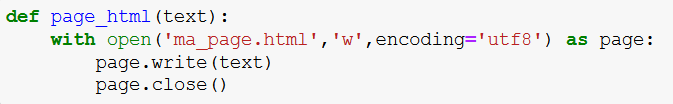
\includegraphics[scale=0.7]{img/python-open.png}
\end{center}
\begin{enumerate}
\item Recopier cette fonction sur votre feuille de programmes.
\item Créer le fichier \textbf{page.html} avec le contenu de la variable \textbf{page} puis vérifier qu'elle s'affiche correctement dans un navigateur.
\end{enumerate}


\item Effectuer une requête GET en passant en paramètre le mot \textbf{internet}. Afficher le code d'état de la réponse HTTP.
\begin{enumerate}
%\item Enregistrer dans la variable \textbf{entete} l'en-tête de réponse du serveur. Afficher la variable.
\item Enregistrer dans la variable \textbf{page} le contenu de la réponse du serveur.
\item Afficher dans le navigateur le contenu de la variable \textbf{page}.
\end{enumerate}


\item On va effectuer une requête POST en passant les paramètres de recherche suivants:
\begin{itemize}
\item mot cherché : internet
\item domaine : algorithmes
\item niveau de lecture facile
\end{itemize}
Pour réaliser cette requête, il faut au préalable enregistrer dans une variable les paramètres de recherche en respectant la structure suivante : {'clef 1' : 'valeur 1', 'clef 2' : 'valeur 2', ... ,'clef n' : 'valeur n'} où les clefs et les valeurs correspondent aux paramètres de recherche.
\begin{enumerate}
\item Enregistrer dans la variable \textbf{p} les paramètres de recherche.
\item Effectuer une requête POST en passant en paramètre la variable \textbf{p}.
\item Enregistrer dans la variable \textbf{page} le contenu de la réponse HTTP du serveur.
\item Afficher dans le navigateur le contenu de la variable \textbf{page}.
\end{enumerate}
\end{enumerate}

\end{document}

